% This file was created by matlab2tikz.
%
%The latest updates can be retrieved from
%  http://www.mathworks.com/matlabcentral/fileexchange/22022-matlab2tikz-matlab2tikz
%where you can also make suggestions and rate matlab2tikz.
%
\definecolor{mycolor1}{rgb}{0.00000,0.44700,0.74100}%
\definecolor{mycolor2}{rgb}{0.85000,0.32500,0.09800}%
%
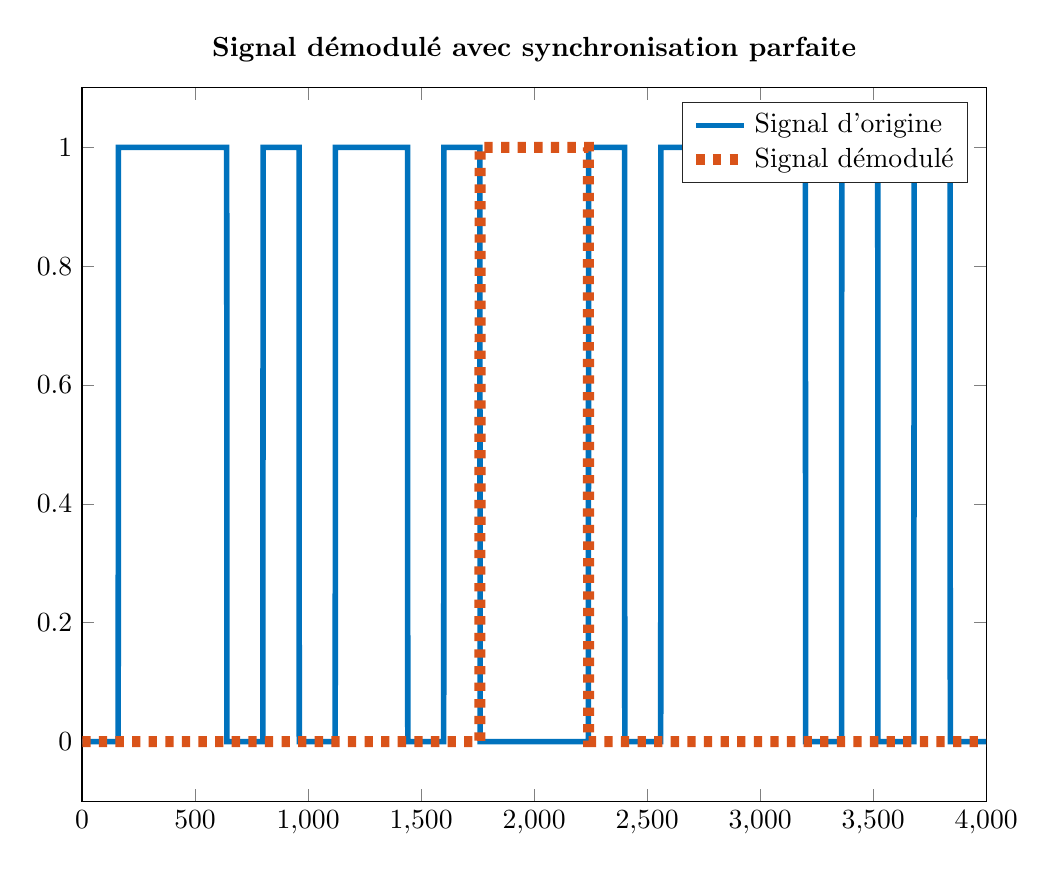
\begin{tikzpicture}

\begin{axis}[%
width=4.521in,
height=3.566in,
at={(0.758in,0.481in)},
scale only axis,
xmin=0,
xmax=4000,
ymin=-0.1,
ymax=1.1,
axis background/.style={fill=white},
title style={font=\bfseries},
title={Signal démodulé avec synchronisation parfaite},
legend style={legend cell align=left, align=left, draw=white!15!black}
]
\addplot [color=mycolor1, line width=2.0pt]
  table[row sep=crcr]{%
1	0\\
160	0\\
161	1\\
640	1\\
641	0\\
800	0\\
801	1\\
960	1\\
961	0\\
1120	0\\
1121	1\\
1440	1\\
1441	0\\
1600	0\\
1601	1\\
1760	1\\
1761	0\\
2240	0\\
2241	1\\
2400	1\\
2401	0\\
2560	0\\
2561	1\\
3200	1\\
3201	0\\
3360	0\\
3361	1\\
3520	1\\
3521	0\\
3680	0\\
3681	1\\
3840	1\\
3841	0\\
4000	0\\
};
\addlegendentry{Signal d'origine}

\addplot [color=mycolor2, dashed, line width=4.0pt]
  table[row sep=crcr]{%
1	0\\
1760	0\\
1761	1\\
2240	1\\
2241	0\\
4000	0\\
};
\addlegendentry{Signal démodulé}

\end{axis}
\end{tikzpicture}%